\paragraph{Definition}
It is \tB{the separating hyperplane that is farthest from the training
observations}. We can compute the (perpendicular) distance from each
training observation to a given separating hyperplane; the smallest
such distance is the minimal distance from the observations to the
hyperplane, and is known as the margin.\\
In a sense, the maximal margin hyperplane represents the mid-line of 
the widest ``slab'' that we can insert between 2 classes.

\begin{figure}[H]
	\begin{center}
		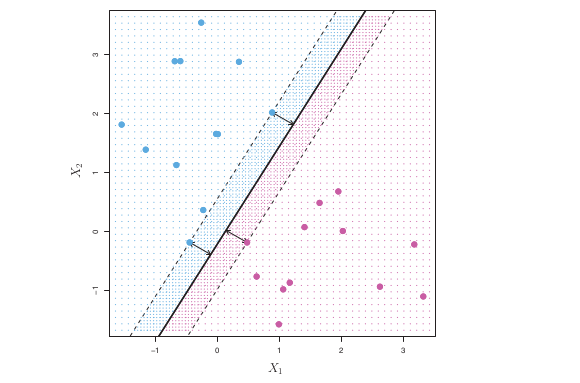
\includegraphics[width=\textwidth]{./chap/1chap/8sec/images/1margineSVM.png}
	\end{center}
	\caption{The margin is distance from the solid line to either
	of the dashed lines. The 2 points and the purple point that 
	lie on the dashed lines are the support vectors}
	\label{fig:8.1margineSVM}
\end{figure}

\paragraph{Construction of the Maximal Margin Classifier}
Set of $n$ observations $
\begin{pmatrix}
	x_{1}
	.
	.
	.
	x_{p}
\end{pmatrix}\in\mathbb{R}^{p}
$ and associated class labels $\prth{y}{i}{n}\in\{-1,1\}$
The maximal margin hyperplane is the solution to the optimization 
problem:
\begin{center}
$ \max\limits_{\prtH{\beta}{i}{0}{p},M}M 
\text{ subject to: }
\begin{cases}
	\su{{j=1}}{p}\beta_{j}^{2}=1~(1)\\
	\forall i\in\inter{1}{n},~y_{i}(\beta_{0}+\su{{j=1}}{p}\beta_{j}x_{ij})>M~(2)
\end{cases} $
\end{center}

(2) \sB{guarantees that each observation will be on the correct side of
the hyperplane, provided that $M\geq 0$}\\

\begin{figure}[H]
	\begin{center}
		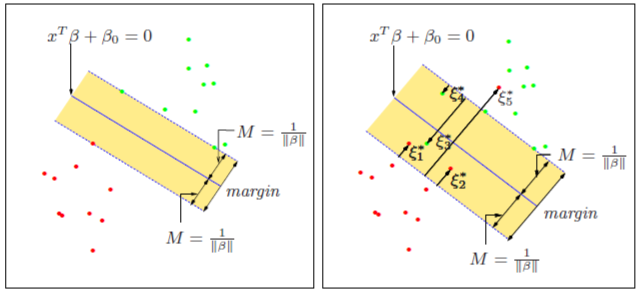
\includegraphics[width=\textwidth]{./chap/1chap/8sec/images/21_svC.PNG}
	\end{center}
	\caption{The left panel shows the separable case. The decision boundary is the solid line,
	while broken lines bound the shaded maximal margin of width $2M=\frac{2}{\norm{\beta}}$.
	The right panel shows the \emph{non-separable} case. The point labeled $\xi_{j}^{*}$ are
	on the wrong side of their margin by an amount $\xi_{j}^{*}=M\xi_{j}$; points on the 
	correct side have $\xi_{j}^{*}=0$. The margin is maximized subject to a total budget
	$\su{}{}\xi_{i}\leq constant$. Hence $\su{}{}\xi_{i}^{*}$ is the total distance of points
	on the wrong side.}
	\label{fig:21_svC}
\end{figure}
We can drop the norm constraint on $\beta$, and instead define $M=\dfrac{1}{\norm{\beta}}$:
$$\min\norm{\beta}\text{ subject to }
\begin{cases}
	\forall i, y_{i}\left(x_{i}^{T}\beta+\beta_{0}\right)\geq M\left(1-\xi_{i}\right)\\
	\xi_{i}\geq 0, \su{}{}\xi_{i}\leq constant
\end{cases}
$$
This is the usual way the support vector classifier is defined from the non-separable case.
\subparagraph{Computing the Support Vector Classifier}
Computationally it is convenient to re-express previous equation:
\begin{center}
\tB{$ \min\limits_{\beta,\beta_{0}}\dfrac{1}{2}\norm{\beta}^{2} + C\su{{i=1}}{N}\xi_{i}\text{ subject
to }\forall i,\xi_{i}\geq 0, y_{i}\left(x_{i}^{T}\beta+\beta_{0}\right)\leq M\left(1-\xi_{i}
\right)$}
\end{center}
where the ``cost'' parameter $C$ replaces the constraint; the separable case corresponds
to $C=\infty$\\
We describe a quadratic programming solution using Lagrange multipliers.
The Lagrange (primal) function is:
\begin{center}
	\enc{$ L_{p}=\dfrac{1}{2}\norm{\beta}^{2} + C\su{{i=1}}{N}\xi_{i}-\su{{i=1}}{N}\alpha_{i}\left[y_{i}^{T}\beta+\beta_{0}-(1-\xi_{i})\right]-\su{{i=1}}{N}\mu_{i}\xi_{i}$}
\end{center}
Setting the respective derivatives to zero we get : 
$
\begin{cases}
	\beta = \su{{i=1}}{N}\alpha_{i}y_{i}x_{i}\\
	0 = \su{{i=1}}{N}\alpha_{i}y_{i}\\
	\alpha_{i} = C-\mu_{i}, \forall i
\end{cases}
$

By inserting the equation system in the Lagrange function we obtain:
$L_{D} = \su{{i=1}}{N}\alpha_{i} - \frac{1}{2}\su{{i=1}}{N}\su{{j=1}}{N} \alpha_{i}\alpha_{j}
y_{i}y_{j}x_{i}^{T}x_{j}$ which gives a lower bound on the objective function (computational 
re-expression) for any feasible point.

